% !TEX TS-program = pdflatex
% !TEX encoding = UTF-8 Unicode

% This is a simple template for a LaTeX document using the "article" class.
% See "book", "report", "letter" for other types of document.

\documentclass[11pt]{article} % use larger type; default would be 10pt

\usepackage[utf8]{inputenc} % set input encoding (not needed with XeLaTeX)

%%% Examples of Article customizations
% These packages are optional, depending whether you want the features they provide.
% See the LaTeX Companion or other references for full information.

%%% PAGE DIMENSIONS
\usepackage{geometry} % to change the page dimensions
\geometry{a4paper} % or letterpaper (US) or a5paper or....
\geometry{margin=1in} % for example, change the margins to 2 inches all round
% \geometry{landscape} % set up the page for landscape
%   read geometry.pdf for detailed page layout information

\usepackage{graphicx} % support the \includegraphics command and options

\usepackage[parfill]{parskip} % Activate to begin paragraphs with an empty line rather than an indent
\setlength{\parindent}{1cm}

%%% PACKAGES
\usepackage{booktabs} % for much better looking tables
\usepackage{array} % for better arrays (eg matrices) in maths
\usepackage{paralist} % very flexible & customisable itemizes (eg. enumerate/itemize, etc.)
\usepackage{verbatim} % adds environment for commenting out blocks of text & for better verbatim
\usepackage{subfig} % make it possible to include more than one captioned figure/table in a single float
\usepackage{amssymb} % more 'unusual' symbols not included in standard LaTeX package
\usepackage{enumitem}
\usepackage{amsmath}
\usepackage{comment}
\usepackage{color}
\usepackage{graphicx}
\usepackage{xspace}
\usepackage{gensymb}
\usepackage{calligra}
\DeclareMathAlphabet{\mathcalligra}{T1}{calligra}{m}{n} 
\DeclareFontShape{T1}{calligra}{m}{n}{<->s*[2.2]callig15}{} 

% These packages are all incorporated in the memoir class to one degree or another...

%%% HEADERS & FOOTERS
\usepackage{fancyhdr} % This should be set AFTER setting up the page geometry
\pagestyle{fancy} % options: empty , plain , fancy
\renewcommand{\headrulewidth}{0pt} % customise the layout...
\lhead{}\chead{}\rhead{}
\lfoot{}\cfoot{\thepage}\rfoot{}


%%% SECTION TITLE APPEARANCE
\usepackage{sectsty}
\allsectionsfont{\sffamily\mdseries\upshape} % (See the fntguide.pdf for font help)
% (This matches ConTeXt defaults)

%%% ToC (table of contents) APPEARANCE
\usepackage[nottoc,notlof,notlot]{tocbibind} % Put the bibliography in the ToC
\usepackage[titles,subfigure]{tocloft} % Alter the style of the Table of Contents
\renewcommand{\cftsecfont}{\rmfamily\mdseries\upshape}
\renewcommand{\cftsecpagefont}{\rmfamily\mdseries\upshape} % No bold!

%%%Command Macros
\newcommand{\vf}{\ensuremath{V_{F}}\xspace}
\newcommand{\sr}{\ensuremath{\mathcalligra{r}} \xspace}
%\newcommand{\sr}{\ensuremath{R_{contact}} \xspace}

%%% END Article customizations

\graphicspath{ {./images/} }

\title{The Mimas Leading Edge Anomaly: Thermal conductivity and grain cementation radius estimation}
\author{M.J. Schaible, R.Johnson, L. Zhigilei}
%\date{} % Activate to display a given date or no date (if empty),
         % otherwise the current date is printed 

\begin{document}
\maketitle

\section{'Abstract': Comparison/Summary of thermal conductivity models}

	\begin{itemize}
	Goals:
	\item Explain the termal condictivity differences between inside/outside anomalous region on Mimas and Tethys
		\begin{itemize}
		\item How can the thermal conductivity differences be explained in terms of structural differences in the regolith
		\item How does the thermal conductivity depend on grain contact, linear or square
		\item Is Hertzian analysis sufficient to determine relative effective contact areas between grains
		\end{itemize}
	\item Estimate effects of $>$1MeV electrons on grain cementation properties
		\begin{itemize}
		\item What is the deposition profile of the electrons in the regolith
		\item How much energy is deposited per interaction
		\item What is the heating effect on $\sim$50$\mu$m grains for each interaction
		\item How many molecules are desorbed from the pore surfaces per interaction
		\item Does the averge number of molecules desorbed vary with depth in the regolith or proximity to pore surface
		\end{itemize}
	\item Estimate time-scale for cementation increase to explain increased cementation
	\item Estimate gardening rate due to micrometeorite bombardment to counteract the sintering process

	Here, several thermal conductivity models are discussed and it is seen that there are qualitative similarities shared by all; namely, that the models depend on the thermal conductivity of bulk ice, $k_{ice}$, the porosity, $\phi$, and on geometric factors that depend on the packing of grains. In each of the models, all contributions to thermal conductivity  other than conduction through grains (i.e. radiative, convective, latent heat) can be shown to be negligible. Conductivity through grains is limited by the contact area between adjacent grains. The models are discussed in more detail in the following and summarized here for ease of comparisson.
	
	\begin{itemize}
	\item Wood (2013)
		\begin{equation}
		k_{eff}  = f_{sc} k_{ice} \frac{\chi + 1 - \phi}{\chi + 1 + \frac{\phi}{2}} \\
		\end{equation}
		
		Where $f_{sc}$ is called the solid continuity factor. It is a measure of the efficiency of contact between adjacent grains and dependent on geometrical packing and contact area, determined by Hertzian analysis and cohesive surface forces (JKR theory), between adjacent grains.
		
		\begin{equation}
		f_{sc} = Y_{sc}N_{c} \left( \frac{N_{c}}{2\sqrt{N_{c}-1}} \frac{R_{con}}{R_{s}} \right)^{Z_{sc}}
		\end{equation}
	
	Here R$_{con}$ is the radius of the contact area, R$_{s}$ is the particle radius, N$_{c}$ is the coordination number, Y$_{sc}$ is determined empirically, Z$_{sc}$ depends on the ratio of solid to void thermal conductivities and, in the case considered here of low temperature and pressure, can be taken to be 1, and the $Y_{sc}$ factor is a fit to experimental data. The coordination number can be calculated exactly for regular packings of monodisperse spheres, with N$_{c}$ = 6 for simple cubic packing, and for small, cohesive, nearly spherical particles Yang et al (2000) gave a functional relationship between coordination number and porosity which closely matches measured and modeled random packings, especially at porosities $\ge$40\%. 
	
	\begin{equation}
	N_{c} = 2.02 \left( \frac{1+87.38(1-\phi)^{4}}{1+25.81(1-\phi)^{4}} \right)
	\end{equation}
		
	Taking $\phi = 0.5$ and assuming $\chi << \phi$ we can simplify this equation to $k_{eff} \approx \frac{2}{5} f_{sc} k_{ice}$. Wood is (apparently) developing an additional model that takes into account the cementation between grains. 
		
%	\item  Piqueuz and Christensen (2009b) \\
%		P and Q did not give explicit equations to calculate the thermal conductivity, but provided several larger plots that traced how the thermal conductivity varied with \% cementation, grain size, gas pressure etc. However, their focus was on ~atm pressure environments, and the model failed for very small grain contact areas (low thermal conductivities), and thus is was determined this model was unfit to explain the regolith at Mimas.

	\item Steiner and K\"{o}mle (1991)
		
		\begin{equation}
		 k_{eff} = \sqrt{1-\phi}\cdot H \cdot k_{ice}(T)
		\end{equation}
		
	Taking $\phi = 0.5$, we can simplify this equation to $ k_{eff} \approx 0.71 H k_{ice}$. The Steiner and K\"omle model uses only the $\sqrt{1-\phi}$ factor to account the the structure of the material. The Hertz factor H is assumed to be similar to the other models. 

	\item Gundlach and Blum (2010)
		
	The Gundlach and Blum model was developed using a mathematical analysis by Chan and Tien (1973) for regularly packed spheres whose contact area is described by Hertzian analysis and where the cohesive forces between spheres are described by JKR theory.
	
		\begin{equation}
		k_{eff} = k_{ice} H \frac{1}{0.531 S(\vf)} \frac{N_{A}}{N_{L}}
		\end{equation}
		
	The factors S$_{vf}$, N$_{A}$, and N$_{L}$ depend on the specific packing arrangement and can be computed explicitly for regular packing arrangements. Note that the porosity of a simple cubic lattice is 47.7\%, close to the 50\% porosity estimated for Mimas. H is the Hertz factor defined as
	
		\begin{equation}
		 H = [\frac{9}{4} \frac{1-\mu^{2}}{E} \pi \gamma r^{2} ]^{1/3}
		\end{equation}
	
	
	\item Sirono and Yamamoto (1997)
		
		\begin{equation}
		k_{eff} = k_{ice} ( \frac{p - p_{c}}{1-p_{c}} )\frac{\pi \sr^{2}}{g r^{2}}
		\end{equation}
		
		Where \sr is the grain contact radius as defined by Hertzian analysis and 'p' is \underline{not} the volume filling factor, but related to it and dependent on the packing. 'p' is the probability that a lattice site is occupied with a regolith grain. The Hertz factor given by Sirono and Yamamoto is slightly different than that of Gundlach and Blum:
		
		\begin{equation}
		H = [ \frac{9 \pi \gamma r^{2} (1-\mu^{2})}{8 E} ]^{1/3}
		\end{equation}
		
	\end{itemize}

\newpage
\section{Introduction}
\label{sec:intro}

	Analysis of Cassini instrument data revealed an anomalous region present on the leading edge of the Saturnian icy moons Mimas and Tethys. The feature was first identified by the VIMS (Visual and Infrared Mapping Spectrometer) instrument as a lens shaped darkening compared to the surrounding regions [Shenketal2011]. It was seen most clearly by taking the ratio of IR/UV light, and the discoloration was centered a 0$\degree$ lat. and 0$\degree$ lon. on the leading edge and extended $\sim \pm30\degree$ to the north and south while spreading over $\>180 \degree$ along the equator. The smaller IR/UV ratio in the anomalous region as compared to surrounding regions was explained as increased scattering at UV wavelengths due to a higher concentration of defects in the icy regolith grains, possibly caused by energetic particle bombardment. Later, using the CIRS (Cassini InfraRed Spectrometer) instrument which measured the thermal IR regime, the emission from the surface was determined during the day and night cycle. Subsequent analysis showed that the temperature variation within a lens shaped region was greater than the surrounding area, indicating a greater thermal conductivity of the material in the lens shaped region, and the spatial extents closely matching the IR/UV discoloration,  [Howettetal2011]. 

	The location of the anomaly was subsequently shown to closely match the expected deposition profile of high energy ($\>$1 MeV) electrons rapidly moving along the magnetic field lines perpendicular to the rotational plane with a high bounce frequency such that they are condenssed out as soon as the magnetic field line crosses the surface. Unlike the thermal plasma, these electrons travel with their net guiding center of motion opposite the rotation direction of the Mimas and Thethys and thereby deposit energy preferentially on the leading edge of these bodies [Paranicasetal2012]. The electons could create scattering centers in the icy regolith which would lead to the observed IR/UV discolorations, and furthermore sintering could lead to increased grain contact and thus explain the anomalous thermal inertia.  The surfaces of the moons are composed almost entirely of crystalline water ice, while essentially free of organic species [Filacchioneetal2010], and the energy deposition due to these electrons was hypothesized to be responsible for an increased sintering volume between the ice grains.

	A good deal of thermal modeling has been done to understand the structure of comets and the thermal inertia of other bodies such as the Moon and Mars. However, the Saturnian moons are composed of water ice as opposed to a rocky regolith and lack the dark organic layer which found on the surface of comets. Also, since the moons lack an atmosphere the thermal conductivity is dominated by intergrain contacts while the thermal conductivity due to gas convection in the regolith is negligible. The purpose of this note is to quantitatively estimate the expected relative contact area or grain sintering radius based on the measured parameters of thermal inertia and grain size. The estimate assumes that both the ice grains and the cementation volume is entirely crystalline. Although amorphous ice could be present, the effect on thermal conductivity of the crystalline to amorphous transition is shown to be a much smaller effect than the increase in surface area. The structure of the ice will be discussed in more detail later in this note. 
	
	%REJ - One nice thing would be to correlate defect production--determing the IR/UV ratio to energy deposition--for which there are expressions and then show that that amount of energy deposition is also consistent with your model of the sintering 

\subsection{Thertmal Inertia ($I$) and Skin Depth ($\delta$)}

		Using the measured surface thermal emission excursions, the values for thermal inertia $I=\sqrt(kc\rho)$ were extracted by Howett et al (2011, 2012). Using the values of thermal inertia and assuming a porosity of $\phi = 50\%$, the thermal conductivity and the skin depths $\delta = \frac{I_{out}}{(1-\phi)\rho_{ice} c \sqrt{\omega}}$ inside and outside the anomalies were determined and are given in table 1, where $c$ is specific heat taken as 0.82 MKS, $\rho_{ice}$ is the density of bulk ice (9340 kg/m$^{3}$), and $\omega$ the angular velocity of rotation. The skin depth of calculated assumes that the conductivity is that of porous, crystalline ice regolith. However, the contact area between grains formed by sintering could have different conductivity. 

	\begin{tabular}[c]{ l | l | c | c | c }
	Body & Location & Thermal Inertia & Skin Depth & Thermal Conductivity \\
	& & $\left[ \frac{J}{m^{2} s^{1/2} K} \right]$ & [cm] & $\left[ \frac{J}{m\cdot s\cdot K} \right]$ \\ \hline
	Mimas & Inside anomaly & 66 $\pm$23 & 2.01 $\pm$0.7 & 1.13 $\left(\substack{+0.94 \\ -0.65} \right) \times$ 10$^{-2}$ \\
		& Outside anomaly & $<$16 & $<$ 0.49 & $<$ 6.7 $\times$ 10$^{-4}$) \\ \hline
	Tethys & Inside anomaly & 25 $\pm$3 & 0.76 $\pm$0.09 & 1.63 $(\pm 0.4) \times$ 10$^{-3}$ \\
		& Anomaly boundary & 11 $\pm$1 & 0.34 $\pm$0.03 & 3.16 $(\pm 0.6) \times$ 10$^{-4}$ \\
		& Outside anomaly & 5 $\pm$1 & 0.15 $\pm$0.03 & 6.53 $\left(\substack{+2.9 \\ -2.4} \right) \times$ 10$^{-5}$ \\
	\end{tabular}

	The average path length traveled by $1 - 10 MeV$ electrons impacting on water, calculated with the ESTAR program using the continuous-slowing-down-approximation (CSDA), is $0.4-5.0 g/cm^{2}$, which for $50\%$ porous water ice gives $0.85-10.6 cm$ total path length [NIST, e-star]. \textcolor{red}{Unfortunately, the NIST data does not give a projected range for the electrons (depth of penetration).} The depth of penetration into the material must be less than the total path length, but due to efficient scattering effects from electron-nucleus and electron-electron interactions, the actual electron penetration depth varies. For light materials such as water ice, the maximum depth is expected to be on the order of the CSDA range [Attix, 2008]. The similarity in the penetration depths of the electrons and the skin depth of the thermal anomaly suggest that the electrons could be responsible for the increased thermal conductivity.  
	
	Here we show that a possible explanation for the thermal conductivity differences could be sintering in an intergrain contact region due to energy deposited in electronic excitations of the water molecules either on the surface or in the bulk of the ice grains. The deposited energy can mobilize water molecules, causing them to migrate along the grain surface or desorb from the surface to be redeposited in the intergrain region. This can lead to grain growth and, more importantly, growth in the size of the contact regions between grains and improved thermal contact  across the grain boundaries.
	
	 As discussed below the same energy deposition that mobilizes the water at the grain boundaries can cause defects in the bulk. Whereas sintering increases the effective thermal conductivity, such defects, which we assume to be the principal cause of the increase in the IR/UV ratio[ref], can cause a decrease in thermal conductivity. However, below we will also show that the density of bulk defects produced at a level consistent with the sintering are sufficient enough to affect the UV scattering but not to significantly decrease the thermal conductivity.
	
%\emph{There should be a pressure minimum in the pendular region. Need equation to explain. Another argument in the minimization of surface energy. Need to look more into that too.}
	
\section{Contributions to the effective thermal conductivity of an icy porous regolith}

	In general, the thermal conductivity of a granular, uncemented sample under vacuum can be separated into a conductive which describes heat flow through the bulk, and a radiative term which describes heat flow through the void space [Watson, 1964]. 
	
	\begin{equation} \label{eq:TCbasic}
	k_{eff} = k_{rad}(T^{3}) + k_{cond}
	\end{equation} 
	
	The first term depends on both grain size and porosity and is due to radiation as dicussed further below. The second factor was given by Watson (1964) as $B = \frac{3000}{D}\times10^{-5}$ for $D > 2m \mu m$ and is a function of the bulk conductivity, $k_{grain}$, and the contact area, $S$, between grains. For porous regoliths typical of airless solar system bodies heat flow is limited by the  amount of intergrain contact.

	In general, $k_{rad}$ and $k_{cond}$ can depend on factors such as grain size, porosity, temperature, gas pressure etc. Thermal conductivity measurments and modelling using either a spherical grain approximation or continuum techniques can be used to parameterize the variables for analitical expressions. However, much work has been done to constrain the various parameters that affect the thermal conductivity, and those possibly relevant to Mimas and Tethys will be outlined and their usefulness for describing the effective thermal conductivities reported by Howett et al, (2011, 2012) is discussed below.
	
%	Computationally, though variations in porosity, vacuum conditions and grain size can be difficult to study in the lab and using solid sphere computational models may miss important effects from the regolith microstructure.

\subsection{Radiative contribution to thermal conductivity}

	The contribution to thermal conductivity from radiative heat emission from the grain/pore surfaces, the first term in \ref{eq:TCbasic}, can be estimated as [(Kasparek and Vortmeyer, 1976)]

	\begin{equation}
	k_{rad} = 4 \psi D \sigma T^{3}
	\end{equation}
	
	where $D$ is the particle diameter, $T$ it the temperature, $\sigma$ is the Stephan Boltzmann constant, and $\psi$ is a heat transport coefficient defined by
	
	\begin{equation}
	\psi = \frac{2F + \epsilon'(1-F)}{2(1-F)-\epsilon'(1-F)}
	\end{equation}

	for which F is a 'radiative constant' equal to $\approx$ 0.08 and $\epsilon'$ is related to the emissivity $\epsilon$ of the material by $\epsilon' = \frac{\epsilon}{\epsilon +0.5(1-\epsilon)}$. Taking $D = 50 \mu m$, and $\epsilon = 1$, then the radiative contribution to the thermal conductivity can be estimated as $k_{rad} \approx 6.3\times10^{-6} \frac{J}{m \cdot s \cdot K}$.
	
	Thus we see that the radiative contribution at appoximate Mimas temperatures can account for only $\approx 1/3000$th of the total thermal conductivity as measured for the anomalous region on Mimas. Though it could account for as much as 1/10th of the thermal conductivity outside of the anomalous region on Tethys, it is typically on the order $<1\%$ contribution to the total thermal conductivity and will be neglected in the remainder of our analysis.

\subsection{Latent heat contribution to thermal conductivity}
	An additional mechanism not considered in \ref{eq:TCbasic} is heat transfer due to molecular desorption and redeposition within pores, i.e. sublimation the expectation being that there is a higher rate of sublimation on the high temperature side of the pore and thus heat conductivity across the void space. We can model the sublimation process using the Hertz-Knudsen formula [ref]:

	\begin{equation}
	k_{lat} = ( \frac{m}{2 \pi k_{B} T})^{1/2}  (L S) \frac{dP}{dT}
	\end{equation}
	
	where $m$ is the mass of the gas molecule, $k_{B}$ is the Boltzmann constant, $L$ is the latent heat of sublimation per unit mass and $S = \phi d$ is the average pore size dimension where $\phi$ is the porosity and $d$ the average particle diameter. $P$ is the vapor pressure of the gas of interest and is given by the Clausius-Clapeyron equation:
	 
	 \begin{equation} \label{eqn:CCpres}
	 P = ae^{(-b/T)}
	 \end{equation}
	 
	 where $a$ and $b$ are experimentally determined parameters given for water vapor over ice by Fanale et al. (1986) as $a = 3.56 \times 10^{12} N m^{-2}$ and $b = 6141.667 K$. Taking the latent heat of sublimation to be $L = 48600 [\frac{J}{mol}]$ and again using a temperature of 80 K, the contribution to thermal conductivity from the latent heat is $k_{lat} = 1.15\times10^{-26} MKS$. Though at low temperatures this effect is negligible, Steiner and K\"{o}mle (1991) showed that it should be included at temperatures above ~170K. At the temperatures considered here the net thermal conductivity of the grains is controlled the second tem in \ref{eq:TCbasic} and is modeled as due to solid state heat transfer.

\subsection{Solid state heat transport models for a porous icy regolith}
	There are several methods in the literature for determining estimating solid state heat transfer in a grainy regolith that take into account grain size, porosity, and a cementation or contact area between adjacent grains. For cold grainy regoliths, heat flow is limited by the intergrain contact area and changes in contact area, cementation crystalline structure and defect structure  cause changes in the thermal conductivity. In the following we will review several approaches to modeling the thermal conductivity of an icy regolith including cementation between grains. 

\subsubsection{What is the Hertz-factor really?}

	In modeling of thermal conductivity of grainy, porous materials, a common approximate technique is to consider a mono- or polydisperse 'bed' of elastic spheres. The requirement for the spheres to be elastic and not a perfect hard sphere stems from physical considerations, since the contact point of hard spheres is infinitesimal, through which no heat can flow. Therefore, the spheres must deform slightly at the contact point so there is some finite area across which heat can flow. At the atomic scale, the heat transfer through disimilar spheres with no adhesive bonding is due predominantly to the van der Waals intereactions which mediate the phonon transfer, while for cemented grains where there is adhesive material connecting the grains which tranfer heat directly through lattice vibrations. Deformation between curved, elastic surfaces in contact was first studied by H. Hertz in 1882, and Hertzian analysis can be used to determine the radius of the intergranular contact area, /sr, and indentation depth of the surfaces. 

	\begin{equation}
	H(r_{g},T) = [\frac{3}{4} \frac{1 - \mu^{2}}{E(T)} F(r_{g}) r_{g}]^{1/3}
	\end{equation}

	where $\mu$ and $E(T)$ are Poisson's ratio and Young's modulus of the material, respectively, and $F(r)$ is an applied force which determines how strongly adjacent particles are bonded. For a loose regolith, the weight of the grains can be used to determine the force and thus the contact area. However, gravitational forces are negligible in the near surface region as compared to the van der Waals bonding calculated by JKR theory [Johnson et al (1971)] which provides orders of magnitude greater adhesive forces.
	 
	 \begin{equation}
	 F_{JKR} = 3 \pi \gamma r_{g}
	 \end{equation} 
	 
	 where $\gamma(T)$ is the specific surface energy of the material and a measure of the adhesive bonding strength between grain surfaces. It should be noted here that this expression may differ substantially for sintered grains where the boundary may have some degree of crystalline bonding.Substituting this expression, we can define the Hertz-factor as the ratio of the effective (regolith) thermal conductivity and the bulk conductivity.
	 
	 \begin{equation}
	 \label{eq:hertz}
	 H(r, T, \vf) = [\frac{9}{4} \frac{1-\mu^{2}}{E(T)} \pi \gamma(T) r_{g}^{2} ]^{1/3}
	 \end{equation}

	Regardless of the actual mechanical properties, an Hertz-factor parameter can be inserted into thermal conductivity expressions to describe the effective radius of the intergranular contact area. A larger Hertz-factor corresponds to greater interparticle contact, thereby allowing a greater heat flux and a higher thermal conductivity. Thus, for otherwise identical regoliths, the Hertz factor is a parameter that can be used to describe the relative amount of intergranular contact for rigid grains. 

	One of the major differences in the following models is that some include the Hertz factor (contact area radius) to only the first power (Wood, Gundlach and Blum), while the other models include the square of the contact radius (Steiner and K\"{o}mle, Sirono and Yamamoto).


\subsubsection{Grain size comparisson via. Hertz-factor analysis}
	
	By taking the Hertz-factor to be the ratio of the effective and bulk thermal conductivities $H = k_{eff}/k_{ice}$ and assuming other materials parameters ($\mu, E, \gamma$) as well as the packing structure are the same inside and outside the anomaly, the ratio of the grain size inside and outside the anomaly necessary to determine the measured thermal conductivity differences can be determined. At lower temperatures where radiative heat transfer is negligible, the thermal conductivity $k_{eff} \varpropto r^{-1/3}$ and will increase with decreasing particle size, possible due to the increased number of interparticle contacts. Taking the ratio of the grain sizes inside at outside the anomaly on Mimas, we find:
	
	\begin{equation}
	 \frac{r_{g,in}}{r_{g,out}} = (\frac{H_{out}}{H_{in}})^{3} = \fbox{0.00013}
	 \end{equation}

	This comparison estimates that the particle size within the anomaly is ~4 orders of magnitude smaller than the particle size outside the anomaly, while comparisons of the measured grain size yield at most a factor of eight difference. Therefore, we conclude that the variation in thermal conductivities does not depend significantly on grain size differences.

\subsubsection{Continuum Modeling}

	 Intergrain conduction was studied by Piqueux and Christensen (2009) using a finite element code and assuming a cemented region connecting grains. Though they were primarily concerned with the effect of gas pressure in the voids between grains, but their results also considered low gas conductivities ($<1x10^{-5}$) which approach the thermal conductivity of a regolith in a vacuum.
	
	\begin{figure}
	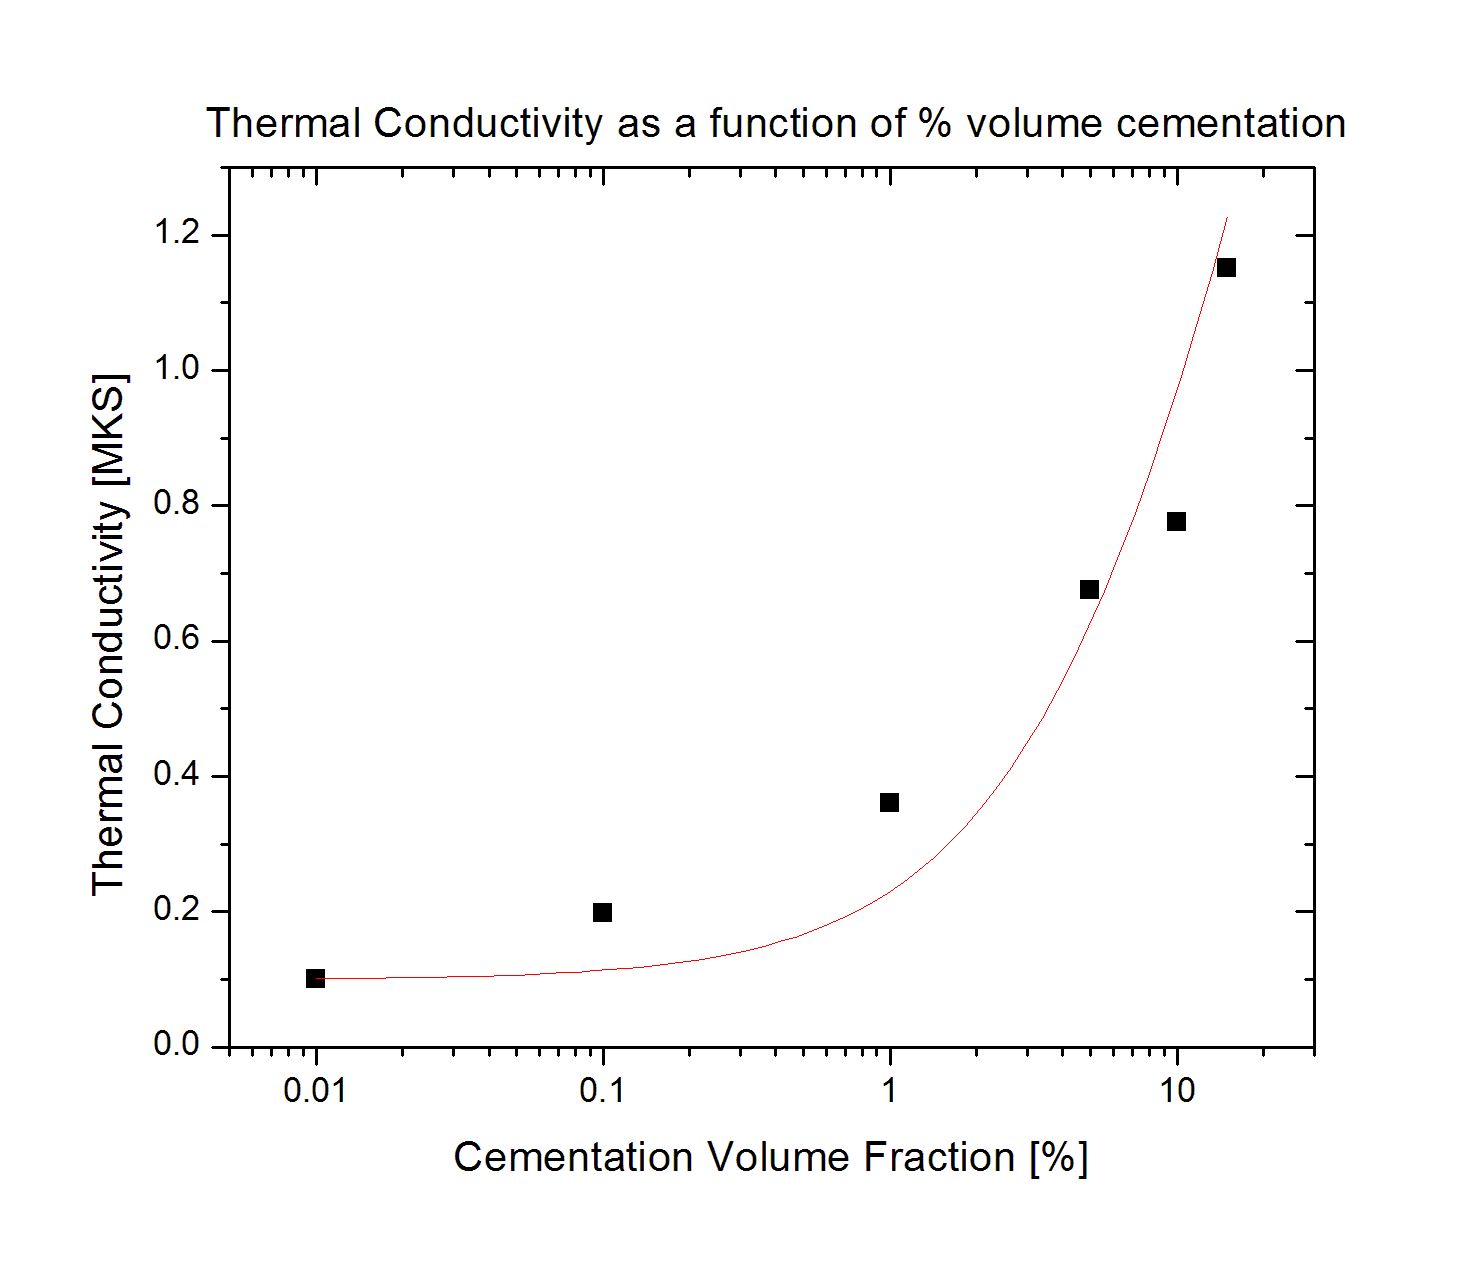
\includegraphics[scale=0.5]{PandQ2009b_CemVolumeFraction.png}
	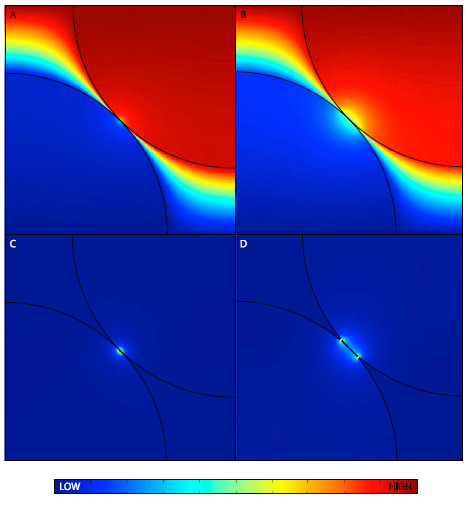
\includegraphics[scale=0.25]{PandQ2009b_Temp_grainimage.png}
	\end{figure}

	The image shows that the thermal conductivity of the anomalous region on Mimas ($k_{in} = 0.0113$ MKS) falls well below the minimum cement volume fraction used by P and C, not including zero cementation. However, it can be seen that, for vanishing gas conductivity,  the relationship between the cement volume fraction and thermal conductivity can be approximated by $V_{cem} \varpropto 21\cdot k_{eff}^{3.32}$ which yields a the volume fraction, $\chi$, of cement inside the anomaly as $<1\times10^{-6} \%$.
	
	It should be noted that the grain thermal conductivity used was 0.937 MKS while the cement thermal conductivity was 6 MKS., and the parcking structures investigated were all cubic regular packings. They show that for very low cement volume fractions the cement thermal conductivity, which should work to increase heat transfer between grains by creating a larger, more continuous bond networks for phonons to travel, is negligible and the effective thermal conductivity, for the ranges evaluated, approaches a single value dependent on grain size and pore gas pressure. Though the effect of varying the grain thermal conductivity was not discussed in the paper, it can be assumed to be negligible because heat transfer between grains is limited by the point of contact between grains. Since small cementation volume fractions of the order estimated by extrapolation were not considered, we cannot use the model of P and C to model the small effects of electron heating of grains and small cementation volumes between grains that are expected due to the low thermal conductivies of Mimas and Tethys. 

\subsubsection{Wood (2011, 2013): Empirical fitting and packing dependencies}
	 Wood (2011, 2013) modeled heat transfer through a grainy porous regolith as being due to conduction through grains and gas filled pores and radiation from grain surfaces across pores, with each thermal path acting in parallel so that $k_{eff} = k_{rad} + k_{cond}$ as in \ref{eq:TCbasic}. Taking $k_{rad}$ to be negligible, as discussed above, Wood further broke down the conductive contribution so that it would lie between a minimum determined by the gas conductivity and a maximum value dependent on solid state conduction.
	
	\begin{equation}
	k_{cond} = k_{c,min} +f_{sc}(k_{c,max}-k_{c,min})
	\end{equation}
	
	Here, $k_{c,min}$ represents the minimum thermal conductivity for the gas phase which, for the low pressure environments of Mimas and Tethys, can be taken to be zero. $k_{c,max}$ depends on the thermal conductivity of the grain material,$ k_{s}$, the porosity $\phi = (1-\nu_{s})$, the volume percent and thermal conductivity of cementation region, $\chi$ and $k_{cem}$ respectively, and  $f_{sc}$ is the fractional continuity of the solid phase and is discussed further below. Wood, 2011 gives the expression
	
	\begin{equation}
	k_{c,max} = \frac{k_{cem}\chi + k_{s}\nu_{s}\frac{3k_{cem}}{2k_{cem}+k_{s}}}{\chi +\nu_{s}\frac{3k_{cem}}{2k_{cem}+k_{s}}+\phi\frac{3k_{cem}}{2k_{cem}}}
	\end{equation}

	Assuming that both the cementation region and the bulk grains are crystalline ice, $k_{s} = k_{cem} = k{ice}$, this can be simplified and the effective thermal conductivity estimated as
	
	\begin{equation}
	k_{eff}=2 f_{sc} k_{ice} \frac{1-\phi}{2+\phi}
	\end{equation}
	
	The $f_{sc}$ factor represents the effect of interparticle contact and/or cementation and is a measure of the efficiency of contact between adjacent grains. The factor contains both geometrical and contact area considerations and, for uncemented soils, is given in terms of the size and number of contacts per particle, where contact size is determined by Hertzian analysis and cohesive surface forces (JKR theory).
	
	\begin{equation}
	f_{sc} = Y_{sc}N_{c} \left( \frac{N_{c}}{2\sqrt{N_{c}-1}} \frac{R_{con}}{R_{s}} \right)^{Z_{sc}}
	\end{equation}
	
	where R$_{con}$ is the radius of the contact area, R$_{s}$ is the particle radius, N$_{c}$ is the coordination number, Y$_{sc}$ is a factor determined by fitting to experimental data, and Z$_{sc}$ depends on the ratio of solid to void thermal conductivities and, in the case considered here of low temperature and pressure, can be taken as 1. The coordination number can be calculated exactly for regular packings of monodisperse spheres, with N$_{c}$ = 6 for simple cubic packing which has a porosith of 47.64\%, similar to the porosity used here. For polydisperse mixtures of randomly packed particles the coordination number cannot be known exactly, but for small, cohesive, nearly spherical particles Yang et al (2000) gave a functional relationship between coordination number and porosity which closely matches measured and modeled random packings, especially at porosities $\ge$50\%. 
	
	\begin{equation}
	N_{c} = 2.02 \left( \frac{1+87.38(1-\phi)^{4}}{1+25.81(1-\phi)^{4}} \right)
	\end{equation}
	
	Using a porosity of 50\%, we find the coordination number is N$_{c}$ = 4.99. We note that for non-spherical particles the shape, orientation, and roughness of a particle can have an effect on the number of contacts and thus the porosity is less strongly coupled to the coordination number. The equilibrium contact radius between two elastic spheres of the same radius R$_{s}$ under a mechanical load can be calculated from JKR theory (Johnson et al., 1991) and is discussed in more detail for non-spherical particles by Wood (2013). The Y$_{sc}$ parameter was fit Wood (2013) for a variety of glass bead samples of various size distributions, yiedling an averaged best fit value of Y$_{sc}$ = 0.09 with a mean standard deviation of 13.6\%. Using these values and assuming a mean particle size of 50$\mu$m, we can determine the solid continuity factor and the contact radius. These values are given in table 2. 

	Taking the ratio of the contact radius values obtained from the Wood analysis, we find $\frac{R_{cont,in}}{R_{cont,out}} = 16.9$ for Mimas, while for Tethys we find $\frac{R_{cont,in}}{R_{cont,out}} = 25.0$. Interestingly, if we take the square root of these values, we find they match closely with the values obtained below. \emph{The Wood model depends only linearly on contact radius, while in reality it should be contact area.}
	
\subsection{Gundlach and Blum, 2012: Hertz factor and packing dependence}

	For packed spheres under vacuum ($k_{cond} = 0$), the heat conductivity can be calculated by [ChanTien1973]:
	
	\begin{equation}
	k_{eff}(r_{g}, T, \vf) = k_{ice}\cdot \sr \cdot \xi(r_{g}, \vf)= k_{ice}(T) H(r_{g},T, \vf)
	\end{equation}

	 where $r_{g}$ is the particle radius, $k_{ice}$ is the thermal conductivity of bulk (solid) ice, \sr is the contact radius, and the packing structure of the material and the number of interparticle contacts is taken into account by $\xi(r, \vf)$ 

	\begin{equation}
	\xi(r_{g}, \vf) = \frac{1}{0.531 S(\vf)} \frac{N_{A}(r_{g})}{N_{L}(r_{g})}
	\end{equation}

	Here, $s(\vf)$ is a 'model parameter' that depends on the packing structure, and $N_{A}(r_{g})$ and $N_{L}(r_{g})$ are the number of particles per unit area and unit length respectivenly. Applying JKR theory (as described below), we can define the Hertz-factor as the ratio of the effective and bulk thermal conductivities which is slightly different than the Hertz factor described in the next section. 
	 
	\begin{equation} \label{eq:GBHertz}
	H(r_{g}, T, \vf) = [\frac{9}{4} \frac{1-\mu^{2}}{E(T)} \pi \gamma(T) r_{g}^{2} ]^{1/3} \xi(r_{g}, \vf)
	\end{equation}
	
	The constants used in the packing structure dependence were only given for regular packing arrangments, and thus could not be used to the random packing considered here. Thus, the analysis of Gundlach and Blum is excluded from further analysis. 
	
\subsection{Determination of grain sinter radius by Hertz factor analysis}

	A third method of determining the effective thermal conductivity of a porous water ice regolith at low pressure (high Knudsen numbers) was outlined in Steiner and K\"{o}mle (1991) who used expressions given in Tsostas and Martin (1987) to derive:

	\begin{equation}
	k_{eff} = (1-\sqrt{1-\phi})\phi \cdot k_{void} + \sqrt{1-\phi}[H k_{ice}+(1-\phi)\frac{B+1}{B}\frac{k_{ice}k_{void}}{k_{ice}+k_{void}}]
	\end{equation}
	
	where $\phi$ is the regolith porosity, $k_{void}$ is the thermal condictivity across the void region due to a combination of radiative heat transfer and the latent heat of sublimation, $k_{ice}$ is the thermal conductivity of bulk ice, $H$ is the 'Hertz-factor' used to describe the radius of the intergrain contact area, and B is a deformation factor related to porosity by:
	
	\begin{equation}
	B = 1.25 ( \frac{1-\phi}{\phi} )^{10/9}
	\end{equation}
	
%	Note that for a porosity of $\phi = 0.5$, the deformation factor $B = 1.25$. Using the greater value of $k_{void} = 6.3\times10^{-6} \frac{J}{m \cdot s \cdot K}$ from the analysis above and a thermal conductivity for ice at 80 K of $k_{ice} = 567/T = 7.09 \frac{J}{m \cdot s \cdot K}$, we can analyze the effective thermal conductivity to obtain a comparison of the Hertz factor inside and outside the thermal anomally feature.

	Taking the thermal conductivity of the void region to be negligible as discussed above, we can simplify the effective thermal conductivity to depend only on the Hertz factor and the porosity of the regolith.
	
	\begin{equation}
	\Rightarrow k_{eff} \approx \sqrt{1-\phi}\cdot H \cdot k_{ice}(T)
	\end{equation}
	
	Using the effective thermal conductivities obtained above for a 50\% porous regolith both inside and outside the anomalies and taking the thermal conductivity of water ice at 80Kto be $k_{ice} = 567/T = 7.09$ MKS [Kossacki et al., (1994)], we can solve for the Hertz-factor. Here it is worthwhile to note that Hertz-factors used previously in the literature to describe a porous icy cometary nucleus are on the order of  $H  \approx (1 - 4) \times10^{-3}$ [SteinerKomle1991], which compares favorably with the values obtained for the Mimas regolith. 

	The following equation is given in Kossacki et al (1994) where it was assumed that the thermal conductivity depended on the square of the contact radius, while it depended linearly on the Hertz factor. If $\sr_{n}$ is the cementation (pendular ring) neck radius and $H_{0}$ is the initial Hertz factor. 
	
	\begin{equation}
	H = H_{0} (\frac{\sr_{n}}{\sr_{n,0}})^{2} \\
	\end{equation}
	
	If we take the 'initial' value to represent the regolith outside of the anomalous region, we have:
	
	\begin{equation}
	\Rightarrow \frac{\sr_{n, in}}{\sr_{n, out}} = (\frac{H_{n, in}}{H_{n, out}})^{1/2}
	\end{equation}
	
	Using this equaion, we find for$\frac{\sr_{n, in}}{\sr_{n, out}} = 4.17$ Mimas and $5$ for Tethys, meaning the effective radius of contact, assuming elastic spheres which deform at the contact point, is greater inside the anomalies that outside and of the same order for the two bodies.
	
\subsection{Effective Medium Theory approach}

	Sirono and Yamamoto (1997), using effective-medium theory, estimated the effective thermal conductivity for a random network of spherical grains arranged on a regular lattice. Integrating the propability distribution of $k$ multiplied by the 1-D heat flux to obtain the effective heat flux yields (Eq. 8 of Sirono and Yamamoto):
	
	 \begin{equation}
	 \frac{k_{eff} - k_{ice}}{k_{ice} +(1/p_{c}-1)k_{eff}}p + \frac{k_{eff}-k_{void}}{k_{void}+(1/p_{c}-1)k_{eff}}(1-p)=0
	 \end{equation}

	 where the probability of a lattice site being occupied or packing fraction is $p$, $p_{c}$  is the percolation thereshold which defines the minimum packing fraction for a continuous thermal path to exist across the material, and $k_{eff}$, $k_{ice}$, and $k_{void}$ are the effective, bulk ice, and void space thermal conductivities respectively. If we take $k_{void} \approx 0$, this equation reduces to:

	\begin{equation}
	k_{eff} = k_{ice} \frac{p - p_{c}}{1 - p_{c}}
	\end{equation}
	 
	 However, this expression does not consider the limitation of heat flow due to reduced area at the grain contacts. This effect can be taken into account by multiplying by a factor dependent on packing structure, grain size and effective contact radius as defined by Hertzian analysis.
	 
	\begin{equation}
	k_{eff} = k_{ice} ( \frac{p - p_{c}}{1-p_{c}} )\frac{\pi \sr^{2}}{g r^{2}}
	\end{equation}

	The analysis of Sirono and Yamamoto discusses the contact area explicitly. Assuming a simple cubic packing structure of the grains, the given the relation between porosity and the packing fraction was 
	
	\begin{equation}
	p = [ \frac{4}{3} \pi ( \frac{1}{2})^{3} ]^{-1} (1 - \phi) \\
	\end{equation}
	
	and the critical packing fraction $p_{c} = 1/3$, and $g = 4$. The calculated contact areas are given in table 1. Of course, since $S = \pi \sr^{2}$, we can calculate the ratio of the contact radius inside and outside the anomaly and find $\frac{\sr_{in}}{\sr_{out}} = ( \frac{S_{in}}{S_{out}} )^{1/2} = 4.14$ for Mimas and $5.0$ for Tethys which is in very close argreement with the value obtained from the analysis of Kossacki et al.

	
\section{Contact radius estimates based thermal conductivity models}

\subsection{Using the Hertz-factor to compare cementation radius}

	\hspace{-2 cm}{
	\begin{tabular}[ l ]{ l | l | c | c | c | c | c }
	\multicolumn{2}{c | }{Authors} & Howett (2011, 2012) & \multicolumn{2}{ | c |}{Wood (2013)} & S\&K (1991) & S\&Y (1997) \\ \hline
	& Location & $k_{eff} \left[ \frac{J}{m\cdot s\cdot K} \right]$ & $f_{sc}$ & $R_{con} [\mu m]$ & H [cm$^{-1/3}$] & S [$\mu m^{2}$]\\  \hline
	Mimas & Inside anomaly & $1.13 \times 10^{-2}$ & $3.98 \times 10^{-3}$ & 0.354 & $2.25 \times10^{-3}$ & 17.1 \\
		& Outside anomaly & $< 6.7 \times 10^{-4}$ &  $2.36 \times 10^{-4}$ & .021 & $1.3 \times10^{-4}$ & 1.00 \\ \hline
	Tethys & Inside anomaly & $1.63 \times 10^{-3}$ &  $5.75 \times 10^{-4}$ & 0.051 & 3.25 $\times10^{-4}$ & 2.47 \\
		& Anomaly boundary &  $3.16 \times 10^{-4}$ &  $1.11 \times 10^{-4}$ & 0.028 & 6.30 $\times10^{-5}$ & 0.48 \\
		& Outside anomaly & $6.53 \times 10^{-5}$ &  $2.30 \times 10^{-5}$ & 0.006 & 1.30 $\times10^{-5}$ & 0.01 \\
	\end{tabular} }

	For all analyses, we see that the contact area inside the anomalous region is greater than without, which is in agreement with the increased thermal conductivity for all other factors being constant.	

\section{Energy deposition due to >1 MeV electrons and Ice Grain Sintering}

	Paranicas et al (2012) estimated the energy flux of electrons deposited on the leading hemispheres of Mimas and Tethys to be $1.21\times 10^{12} \frac{eV}{cm^{2}\cdot s}$ and $1.91\times 10^{11} \frac{eV}{cm^{2}\cdot s}$ respectively.
	
	Kossacki et al (1994) gave an estimate for the neck growth rate due to vapor transport driven by thermal desorption from the grain surface. This is the dominant sintering mechanism at $\sim$200K (see Thomas, 1992), though it may not be relevant at Mimas surface temperatures.
	
	\begin{equation}
	\frac{dr_{n}}{dt} = \frac{\Omega^{2}\gamma p A}{(2\pi\mu RT)^{1/2}RT} \left( \frac{2}{r_{g}} + \frac{1}{\rho} - \frac{1}{r_{n}} \right)
	\end{equation}
	
	where $\Omega$, $\gamma$, and $\mu$ are the molar volume, surface energy, and molar mass of water ice, respectively, $r_{n}$ is the neck radius, $r_{g}$ is the grain radius. The pressure $p$ due to sublimation of molecules from the pore surfaces can be calculated using the Clausius-Clapeyron equation given earlier (\ref{eqn:CCpres}), and the the neck surface area is given by
	
	\begin{equation}
	A = 4\pi\rho \left[ (r_{n} + \rho)arcsin\left(\frac{r_{a}}{\rho}\right) - r_{a} \right]
	\end{equation}
	
	where $r_{a}$ and $\rho$ are defined by
	
	\begin{equation}
	\rho = \frac{r_{n}^{2}}{2(r_{g}-r_{n})}
	\end{equation}
	
	and
	
	\begin{equation}
	 r_{a} = \frac{r_{g}\rho}{r_{g}+\rho}
	\end{equation}
	
	\emph{I think the goal here should be to relate the warming of the grain due to a electron ineratction with the regolith to a average desorption rate. I am imagining this as the number of electeron interactions per surface area per time, multiplied by an average number of desorbed molecules per event to give number of desorbed molecules per area per time.}
	
	Steiner and K\"{o}mle (1993) gave the energy balance at the surface of an uncovered, porous water ice regolith as
	
	\begin{equation}
	S = \left( - k_{eff} \frac{\partial T}{\partial z} \right) + Z^{w}L^{w} +\epsilon \sigma T_{surf}^{4}
	\end{equation}
	
	where $S$ is the energy flux incident on the surface of the regolith, $Z^{w}$ is the free sublimation rate of water ice given by the Hertz-Knudsen formula, $L^{w}$ is the latent heat of water ice, and $\epsilon$ is the IR emissivity. The Hertz-Knudsen formula gives the rate of phase change for a given interface. For a low pressure solid/vapor boundary such as that considered here, this rate of molecular desorption was estimated by Tschudin (1946) as
	
	\begin{equation}
	Z^{w} = P_{s}(T)\frac{\mu}{\sqrt{2\pi R T}}
	\end{equation}
	
	where $P_{s}(T)$ is the saturation vapor pressure.
	
	What is the expected heating rate/area per electron interaction with the ice? How close does the interaction have to be to the surface to desorb a water molecule? What is the primary knock-on sputtering contribution?
	
The electronic structure of ice at the interface of large porous cavities in amorphous ice may resemble that of the free surface interface, and therefore it might be expected that ESD processes would occur there with similar mechanisms. The total ESD neutral product yields are generally much higher from amorphous ice than from crystalline. This is attributed to increased
defect density and an increase in excitation localization due to disruption of long range order in the matrix [Sieger and Orlando, Surf. Sci. 451(2000) 97]

\newpage

\section{Appendiux 1: Review of measured Parameters}
\label{sec:measured}

\subsection{Thermal Inertia (I) - Howett et al. (2011)}
\label{sec:inertia}

	\begin{equation}
	I = \sqrt{kc\rho} \: [\frac{J}{m^{2} K^{1} s^{1/2}}]
	\end{equation}

	\hspace{1cm}
	Where
	\begin{itemize}[leftmargin=3cm]
	\item k = thermal conductivity $[\frac{J}{m \cdot s \cdot K}]$
	\item c = specific heat $[\frac{J}{g \cdot K}]$
	\item $\rho$ = density $[\frac{g}{m^{3}}]$
	\end{itemize}

	The thermal inertial measured by Cassini CIRS was reported by Howett et al. (2011, 2012)
	\begin{itemize}
		\item For Mimas:
		\begin{itemize}
			\item Within anomaly: \fbox{$66 \pm 23  [\frac{J}{m^{2} K^{1} s^{1/2}}]$}
			\item Outside anomaly: \fbox{$< 16  [\frac{J}{m^{2} K^{1} s^{1/2}}]$}
		\end{itemize}
		\item For Tethys:
		\begin{itemize}
			\item Within anomaly: \fbox{$25 \pm 3$ MKS}
			\item Anomaly boundary: \fbox{$11 \pm 1$ MKS}
			\item Outside anomaly: \fbox{$5 \pm 1$ MKS}
		\end{itemize}
	\end{itemize}
		
	\emph{Depth of penetration for CIRS wavelength light?}
	
\subsection{Temperature ranges - Howett et al. (2011)}
\label{sec:temperature}

	Estimated Mimas daytime temperatures: 40-95 K
	
\subsection{Average Particle Size}
\label{sec:size}

%In the UV, Mimas is nearly as bright as Enceladus. Tethys is surprisingly dark in the UV.
%Modeling (Hamilton and Burns, 1994) showed that e-ring grains at the orbit of Mimas (inside the 3.95 R$_{s}$ orbit of Enceladus) are expected to coat the trailing hemisphere of the moon, while at Tethys and other satellites exterior to Enceladus, the e-ring grains impact primarily on the leading hemispheres. 
	
Particle size (diameter) measured using the Cassini observations and, assuming pure water ice regoliths, comparing the water ice absorption band depths at 2.0$\mu m$ and 1.52$\mu m$ to a model correlating absorption depth to grain size developed by Clark and Lucey (1984).

	\begin{itemize}
	\item Mimas: (Hendrix et al, 2012)
	\begin{itemize}
		\item Leading hemisphere: 20-80 $\mu$m
		\item Trailing hemisphere: 10-50 $\mu$m
		\item Herschel crater: 50-100 $\mu$m
	\end{itemize}

	\item Tethys: (Fillachione et al, 2012)
	\begin{itemize}
		\item Average: 30 $\mu$m
		\item Pure H$_{2}$O ice: 22 - 880 $\mu$m
		\item Mixed grains: 69 $\mu$m
	\end{itemize}

	\item Dione (assuming pure water ice): (Newman et al, 2009)
	\begin{itemize}
		\item Whispy region: 6-28 $\mu$m
		\item Dark area: 1-8 $\mu$m
		\item Background: 7-28 $\mu$m
	\end{itemize}
	\end{itemize}

\subsection{Porosity}
\label{sec:porosity}

	The density of a porous medium is given by $\rho_{\phi} = \rho_{0}*(1-\phi)$ where $\rho_{0}$ is the density of the bulk substance. 

	\begin{itemize}
	\item For Enceladus - Verbischer et al (2005): $~50-70\%$
	\item For Tethy's - Caravano et al. (2007): $>90\%$ 
	\item Model parameter (ansatz) Leliwa-Kopystynski (2000): $~50\%$
	\end{itemize}
	
\subsection{Density}

\section{List of Variables}
$\phi$ = porosity
$\chi$ = cementation volume fraction
$\nu_{s}$ = solid volume fraction

\section{Tabulated Literature Parameters}
\label{sec:tabulated}
	
\subsection{Thermal Conductivity}
\label{sec:tconductivity}
	
	Low temperature thermal conductivity
	
	\begin{itemize}
	\item Water Ice
		\begin{itemize}
		\item Ellsworty and Schubert (1983): $k_{ice} = \frac{488.12}{T} +0.4685 \: [\frac{J}{m s K}]$
		\item Haruyama et al (1993) via. Sirono and Yamamoto (1997):
			\begin{itemize}
			\item Amorphous: $k_{H_{2}O, a} = k_{ao} \times T$ where $k_{ao} = 7.1x10^{-3} \: [\frac{erg}{cm s K}]$
			\item Crystalline: $k_{H_{2}O, c} = k_{co}/T$ where $k_{co} = 5.67x10^{7} \: [\frac{erg}{cm s K}]$
			\end{itemize}
		\item Kossacki et al. (1994): $k = \frac{567}{T} \: [\frac{J}{m s K}]$
		\item Klinger (1975): $k_{100 K} = 0.04  \: \frac{J}{m s K}$ (amorphous)
		\end{itemize}
%	\item Silicates
%		\begin{itemize}
%		\item Basalt
%			\begin{itemize}
%			\item Clauser (1995) - Bulk: k $\approx 1.5 - 3.5 [ \frac{J}{m \cdot s \cdot K}]$
%			\item Fountain and West (1970) - Crushed (37-62 $\mu m, \rho = 0.9 g/cm^{3}$, T=150K): k $\approx 7\times10^{-4} [\frac{J}{m \cdot s \cdot K}]$
%			\end{itemize}
%		\item Quartz
%			\begin{itemize}
%			\item engineeringtoolbox.com - Bulk: k $\approx 3.0 [\frac{J}{m \cdot s \cdot K}]$
%			\item Smoluchowski (1910) - Crushed (94$\mu$m): k $\approx 3.0 [\frac{J}{m \cdot s \cdot K}]$
%			\end{itemize}
%		\item Pumice
%			\begin{itemize}
%			\item  Hemmings et al. (2009) - Bulk: k $\approx 0.4269 [\frac{J}{m \cdot s \cdot K}]$
%			\item Wechsler and Glaser (1965) - Crushed (44-104 $\mu$m): 
%			\end{itemize}
%		\end{itemize}
	\end{itemize}

\subsection{Specific  and Latent Heat}
\label{sec:sheat}

	Low temperature specific heat:
	
	\begin{itemize}
	\item Ramirez et al. (2012): $c_{100 K} ~ 0.83 [\frac{J}{g K}]$
	\item NBS Monograph 21 (): $c_{100 K} = 0.82 [\frac{J}{g K}]$
	\item Gutierrez et al. (2001): $c_{H_{2}O} = (0.9 + 0.00749 * T) [\frac{J}{g K}]$
		$\rightarrow c_{H_{2}O}(80K) = 1.50 J/g\cdot K$
	\end{itemize}
	
	Latent heat of sublimation:
	
	\begin{itemize}
	\item Gutierrez et al. (2001): $L = 48600 [\frac{J}{mol}]$
	\end{itemize}

\section{Appendix 2: Calculations}

\begin{itemize} 
\item Skin Depth (calculated for Mimas - outside anomaly)
\begin{equation}
\begin{split}
\delta_{out} &= \frac{I_{out}}{\rho_{regolith} c \sqrt{\omega}}  \\
&= \frac{I_{out}}{(1-\phi)\rho_ {ice} c \sqrt{\omega}} \\
&= \frac{16[\frac{J}{m^{2} s^{1/2} K}]}{(1-0.5)0.934[\frac{g}{cm^{3}}]0.8[\frac{J}{g \cdot K}]\sqrt{7.7\time10^{-5}[\frac{rad}{s}]}} \\
\Rightarrow \delta_{out}&= 0.49\: [cm]
\end{split}
\end{equation}

\item Radiative thermal conductivity
	\begin{equation}
	\begin{split}
	\Rightarrow \epsilon' &= 1 \\
	\Rightarrow \psi &= \frac{1+F}{1-F} \approx 1.087 \\
	\Rightarrow k_{rad} &= 4 (1.087)(5\times10^{-5} m)(5.67\times10^{-8} \frac{J}{m^{2} s K^{4}}(80 K)^{3}) \\
	\Rightarrow k_{rad} &= 6.3\times10^{-6} \frac{J}{m \cdot s \cdot K}
	\end{split}
	\end{equation}

\item Sublimation Heat Transfer
	\begin{equation}
	\begin{split}
	k_{lat} = [ \frac{18 \frac{g}{mol} \times N_{A}}{2 \pi k_{b} (80K)} ]^{1/2} (48600 \frac{J}{mol} & \times N_{A})(0.9 \cdot 50\times10^{-6} m) [ \frac{(3.56\times 10^{12} \frac{N}{m^{2}})(6141.7 K)}{(80 K)^{2}} exp( \frac{-6141.7}{80} ) ] \\
	\Rightarrow k_{lat} &= 1.15\times10^{-26}\frac{J}{m \cdot s \cdot K}
	\end{split}
	\end{equation}

\item Wood 2011 simplification
	\begin{equation}
	\begin{gathered}
	k_{c,max} = k_{ice} \frac{\chi + 1 - \phi}{\chi + 1 + \frac{\phi}{2}} \\
	\Rightarrow k_{eff} = f_{sc} k_{c,max} = f_{sc} k_{ice} \frac{\chi + 1 - \phi}{\chi + 1 + \frac{\phi}{2}} \\
	\\
	\text{assuming   } \chi << \phi  \Rightarrow k_{eff}=2 f_{sc} k_{ice} \frac{1-\phi}{2+\phi}
	\end{gathered}
	\end{equation}

\item Steiner and K\:{o}mle 1991 simplification
	\begin{equation}
	\begin{gathered}
	k_{eff} = (1-\sqrt{1-0.5})(0.5)(6.3\times10^{-6}) + \sqrt{1-0.5} [ H \cdot 7.09+(1-0.5)\frac{1.25+1}{1.25}\frac{(7.09)(6.3\times10^{-6})}{(7.09+6.3\times10^{-6})} ] \\
	\Rightarrow k_{eff} = ( 4.93\times 10^{-6} + 2.24\cdot H )  \frac{J}{m \cdot s \cdot K} \\
	\Rightarrow k_{eff} \approx \sqrt{1-\phi}\cdot H \cdot k_{ice}(T)
	\end{gathered}
	\end{equation}

\item Sirono and Yamamoto 1997 expression variations
	\begin{equation}
	\begin{gathered}
	k_{eff}=k_{ice}\left( \frac{p-p_{c}}{1-p_{c}} \right) \frac{\pi \sr^{2}}{gr^{2}} \\
		 =k_{ice}\left( \frac{p-p_{c}}{1-p_{c}} \right) \frac{\pi}{g r^{2}} H^{2} \\
		 = k_{ice}\left( \frac{p-p_{c}}{1-p_{c}} \right) \frac{\pi}{g r^{2}}[ \frac{9 \pi \gamma r^{2} (1-\mu^{2})}{8 E} ]^{2/3}
	\end{gathered}
	\end{equation}
	
\item Sirono and Yamamoto Contact Area
	\begin{equation}
	\begin{gathered}
	S_{in} = \frac{k_{eff, in}}{k_{ice}} \frac{1-p_{c}}{p - p_{c}}\cdot g r_{grain}^{2} \\
	= \frac{0.00113}{7.09} \frac{1-1/3}{0.955-1/3} \cdot (4)(50 \mu m)^2 \\
	\Rightarrow S_{in} = 1.71\times 10^{-11} m^{2} \\
	\Rightarrow S_{out} = 1.00\times 10^{-12} m^{2}
	\end{gathered}
	\end{equation}
	
\item Grain radius simplification
	\begin{equation}
	\begin{split}
	\frac{H_{in}}{H_{out}} &= \frac{k_{in}}{k_{out}} = \frac{r_{in}^{2/3} \xi(r_{in}, \vf)}{r_{out}^{2/3} \xi(r_{out}, \vf)} \\
	\Rightarrow \frac{H_{in}}{H_{out}} &= \frac{r_{in}^{2/3} \frac{N_{A}(r_{in})}{N_{L}(r_{in})}}{r_{out}^{2/3} \frac{N_{A}(r_{out})}{N_{L}(r_{out})}} \\
	& \text{where }\: N_{A}\varpropto \frac{1}{r^{2}} \: \text{and} \: N_{L}\varpropto \frac{1}{r} \\
	\Rightarrow \frac{r_{in}}{r_{out}} &= (\frac{H_{out}}{H_{in}})^{3}
	\end{split}
	\end{equation}

\item Gundlach and Blum 2012 extension of Hertz analysis to aggregates
	 This thermal conductivity equation can be modified to describe a porous regolith layer composed not simply of spherical grains, but of grain aggregates which themsleves are composed of ice grains and which have their own unique materials parameters such as volume filling factor, Poisson's ratio, Young's modulus, and specific surface energy. Taking the volume filling factor of the layer to be the product of the volume filling factors of the aggregates themselves (\vf$_{agg}$) and the volume filling factor of the aggregate structure \vf$_{struc}$), i.e. ($V_{F, layer} = V_{F, agg} V_{F, struc}$, we can write the effective thermal conductivity of the layer as:
	 
	 \begin{equation}
	 \begin{split}
	 k_{layer}(r_{0}, R, T, V_{F, struc}, V_{F, agg}) = \\
	 k_{agg}(r_{0}, T, V_{F, agg}) [\frac{9}{4} \frac{1 - \mu_{agg}^{2}}{E_{agg}(T)}  \pi \gamma_{agg}(T) r^{2}]^{1/3} \xi(R, V_{F, struc})
	 \end{split}
	 \end{equation}
	 
	 where $R$, $E_{agg}$, and $\mu_{agg}$ are the radius, Young's modulus, and Poisson's ratio of the aggregates, respectively. Taking $r_{0}$ to be the grain radius (the size of the grains that make up the aggregate), the specific surface energy of the aggregates can be calculated by:
	 
	 \begin{equation}
	 \gamma_{agg}(T) = V_{F, agg} \gamma_{ice}^{5/3}(T)[\frac{9 \pi (1-\mu_{agg}^{2})}{r_{0} E_{ice}(T)}]^(2/3)
	 \end{equation}
	 
	 The thermal conductivity of the aggregates can be calculated as before:
	 
	 \begin{equation}
	 k_{eff}(r_{0}, T, V_{F, agg} = k_{ice}(T) [\frac{9 (1-\mu_{ice}^{2})}{4 E_{ice}(T)}\pi \gamma_{ice}(T) r_{0}^{2} ]^{1/3}\xi(r_{0}, V_{F, agg})
	 \end{equation}

\end{itemize}
	
\end{document}